\section{Temperature Acquisition Channel}
			
	\subsection{Termperature Sensor}
	
		Since the 19$^th$ century it is known that the junction between two different metals submitted to a heat flow generates a electromotive force. A thermocouple is a device that has this junction of two different metals and has a known voltage generated output proportional to the heat tranfer on the junction. In theory any combination of two different metals could be used, but there are normalized combinations which produces more stable and predictable voltage outputs. \cite{pollock1991thermocouples} This relation between heat transfer and voltage is known not to be linear as Figure \ref{fig-thermocoupleVoltage} shows (E,J,K,T,R,S and B are designators for normalized thermocouples junction types).

		\begin{figure}[htbp]
			\centering
				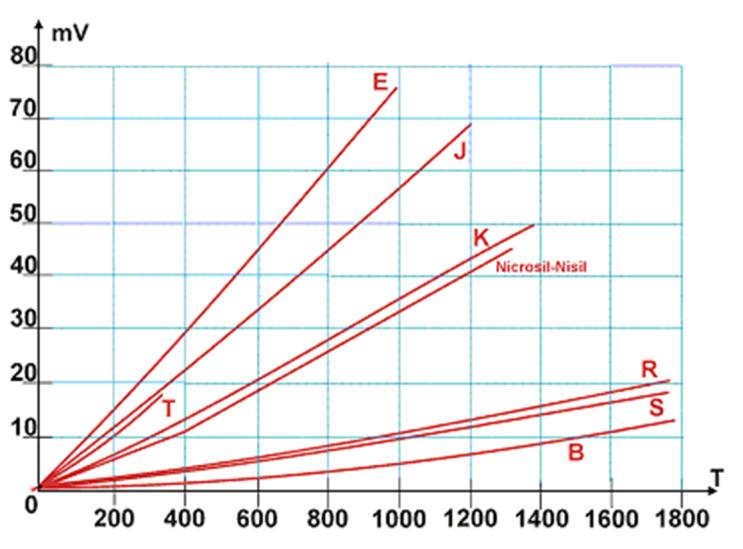
\includegraphics[scale=0.6]{figuras/saida_termopar.jpg}
			\caption{Thermocouple characteristic voltage output \cite{termo-curves}}
			\label{fig-thermocoupleVoltage}
		\end{figure}
		
		Thermocouple actually have two junctions, a hot junction (the one that is submitted to heat transfers) and a cold junction (also called reference junction). What the thermocouple really measures is the difference between the temperature of this two junctions, this means that in a hypothetical situation which the hot junction is submmited to a 100$^{\circ}$C and the cold junction is submitted to a environmental temperature of 25$^{\circ}$C, after thermal equilibrium is reached the thermocouple voltage will be proportional to a temperature of 75$^{\circ}$C. Hence the thermocouple will only produce a "real" output voltage when the cold junction is submitted to a 0$^{\circ}$C (in some calibrations procedures the cold junction is actually submitted to 0$^{\circ}$C) \cite{kinzie1973thermocouple}.
		
		\begin{figure}[htbp]
			\centering
				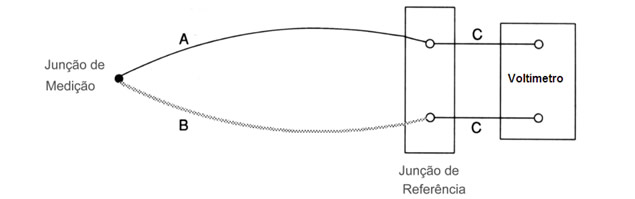
\includegraphics[scale=0.75]{figuras/termoesquema.jpg}
			\caption{Thermocouple Measurement \cite{termo-med}}
			\label{fig-thermocoupleMeasurement}
		\end{figure}
		
		There is a big variety of thermocouples available, table \ref{table-thermocouple} shows the most common thermocouples and there temperature range. For this project it was defined that thermocouples of type K (formed by the junction of two metal leagues: Alumel and Cromel) would be used in this project. This is because this specific type of thermocouple has a wide range of operation (-200$^{\circ}$C - $^{\circ}$C), so according to the requirements they are never too close from the boundary values, a thermocouple of type T or even a type J would not be suitable. Other appealing factor is that this type of thermocouple is quite common so getting eventual replacements would be easier, in comparisson with type E thermocouples.
		 
		\begin{table}[h!]
			\centering
			\caption{Termopares e suas faixas de operação}
			\ref{table-thermocouple}
			\begin{tabular}{|c|c|}
			\hline
			\textit{\textbf{Thermocouple Type}} & \textit{\textbf{Range of Operation ($^{\circ}$C)}} \\ \hline
			J & 0 a 750 \\ \hline
			K & -200 a 1250 \\ \hline
			E & -200 a 900 \\ \hline
			T & -250 a 350 \\ \hline
			\end{tabular}
		\end{table}

	\subsection{Thermocouple Signal Condition}